\textit{Response.} 

\begin{enumerate}[a)]
	\item Below is a plot for a Markov Chain with length $N = 10^4$.
	
		\begin{figure}[H]
			\centering
			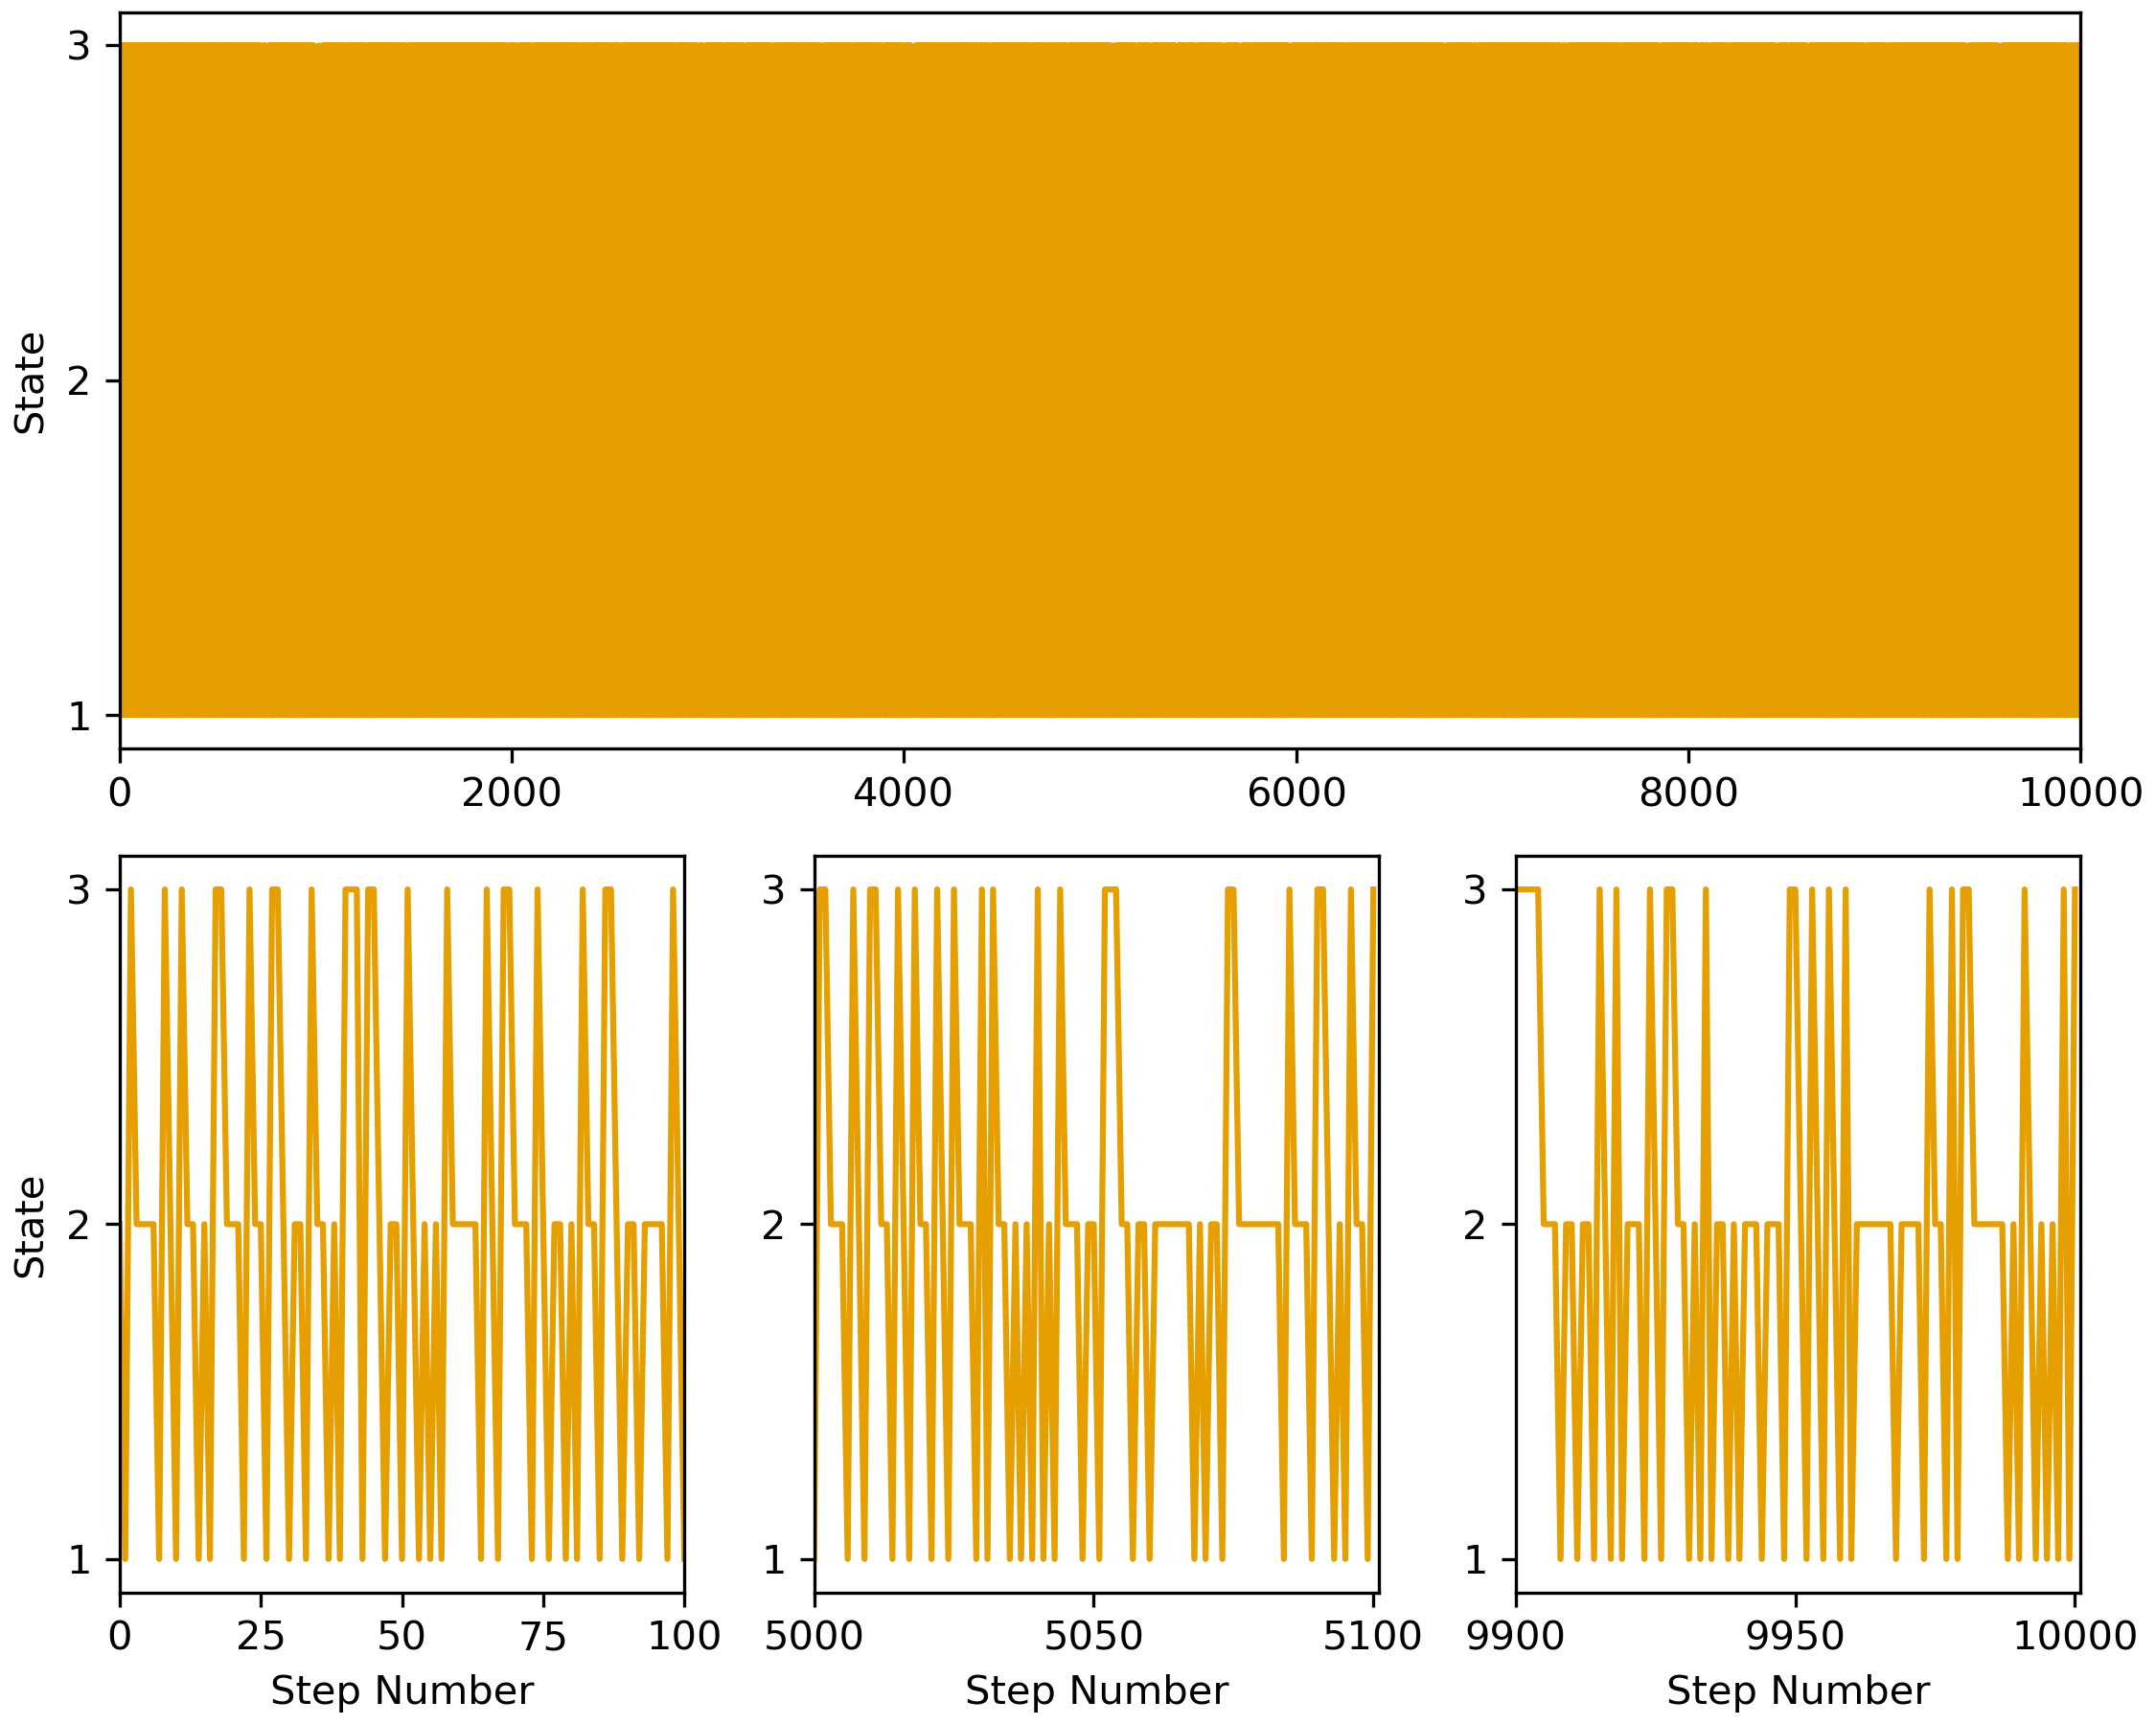
\includegraphics[width=0.75\textwidth]{../../src/1a_traj.png}
			\caption{A sample trajectory for the Markov Chain with transition probability matrix given in Eqn.~\ref{eqn:trns_mtx}. The entire trajectory (top), the first 100 steps (bottom-left), steps 5000 to 5100 (bottom-center), and final 100 steps (bottom-right).}
			\label{fig:traj_1}
		\end{figure}
		
		Source code is available from the GitHub repository
	
	\begin{center}
		\url{https://github.com/jasonltorchinsky/MATH833_HW/releases/tag/hw2}
	\end{center}

	and is given in Appendix~\ref{app:code_1}. In short, the code takes an input parameter \texttt{-{}-N} (or \texttt{-n}) which controls the number of steps the code will simulate. It also accepts and additional flag, \texttt{--do-plot} which will generate a plot of the simulated trajectory, akin to that shown in Figure~\ref{fig:traj_1}. A random initial condition is selected, and each step the next state is randomly chosen according to the conditional distribution $\func{p}{x_n+1\ \vert\ x_{n}}$ defined by the rows of $\vb{P}$.
	
	\item The equilibrium distribution $\va*{\pi}$ of the transition matrix $\vb{P}$ is the unique probability distribution which solves the matrix equation
	
		\begin{equation}
			\va*{\pi} = \va*{\pi}\,\vb{P} \impl \gpr{\vb{\mathcal{I}} - \vb{P}}^T\,\va*{\pi}^T = \vb{0},
		\end{equation}
		
	where $\vb{\mathcal{I}}$ is the identity matrix. In other words, $\va*{\pi}^T$ spans the null space of $\gpr{\vb{\mathcal{I}} - \vb{P}}^T$ and has unit magnitude. The null space of $\gpr{\vb{\mathcal{I}} - \vb{P}}^T$ is spanned by $\va*{\pi}' = \mqty[\frac{9}{8} & \frac{7}{4} & 1]^T$, which we may show through straightforward matrix multiplication
		
		\begin{align}
			\gpr{\vb{\mathcal{I}} - \vb{P}}^T\,\va*{\pi}' &= \mqty[1 & -\frac{1}{2} & -\frac{1}{4} \\[6pt]
																   -\frac{1}{3} & \frac{1}{2} & -\frac{1}{2}\\[6pt]
																   -\frac{2}{3} & 0 & \frac{3}{4}]\,\mqty[\frac{9}{8} \\[6pt] \frac{7}{4} \\[6pt] 1] \nonumber \\
				&= \mqty[\frac{9}{8} - \frac{7}{8} - \frac{1}{4} \\[6pt]
				         -\frac{3}{8} + \frac{7}{8} - \frac{1}{2} \\[6pt]
				         -\frac{3}{4} + 0 + \frac{3}{4}] = \va{0}.
		\end{align}
		
	By dividing $\va*{\pi}'$ by the sum of its entries, we obtain the equilibrium distribution
	
		\begin{equation}
			\va*{\pi} = \mqty[\frac{9}{31} & \frac{14}{31} & \frac{8}{31}].
		\end{equation}
	
	\item Using the final half of a run with $10^4$ steps, we estimate the equilibrium distribution to be $\va*{\pi}^{*} = \mqty[0.29014197 & 0.45790842 & 0.25194961]$. The true equilibrium distribution, to eight decimal points, is $\va*{\pi} = \mqty[0.29032258 & 0.45161290 & 0.25806452]$. The squared-norm of the difference between this estimate and the true value is approximately $7.706 \times 10^{-5}$.
\end{enumerate}
